\documentclass{scrreprt}

\usepackage{aligned-overset}
\usepackage{amsmath}
\usepackage{amsthm}
\usepackage{amssymb}
\usepackage{bm}
\usepackage[inline,shortlabels]{enumitem}
\usepackage{hyperref}
\usepackage[utf8]{inputenc}
\usepackage{multicol}
\usepackage{mathtools}
\usepackage{pdflscape}
\usepackage{physics}
\usepackage{tabularx}
\usepackage[table]{xcolor}
\usepackage{titling}
\usepackage{fancyhdr}
\usepackage{xfrac}
\usepackage{pgfplots}

\pgfplotsset{compat = newest}
\usepgfplotslibrary{fillbetween}
\usetikzlibrary{calc}


\author{Karsten Lehmann}
\date{SoSe 2025}
\title{Übungsblatt 13\\INF-B-120, Mathematische Methoden für Informatiker}

\setlength{\parindent}{0pt}

\setlength{\headheight}{26pt}
\pagestyle{fancy}
\fancyhf{}
\lhead{\thetitle}
\rhead{\theauthor}
\lfoot{\thedate}
\rfoot{Seite \thepage}

\begin{document}
\paragraph{13.1}
\begin{enumerate}[(a)]
\item Gegeben is das homogene lineare Differentialgleichungssystem
  \[
    y'\qty\big(x) = \begin{pmatrix}
      1 & 6 \\
      5 & 2 \\
    \end{pmatrix}y\qty\big(x)
  \]

  Bekannt ist, dass $v_1 = \begin{pmatrix} 1 \\ 1 \end{pmatrix}$ und
  $v_2 = \begin{pmatrix} 6 \\ -5 \end{pmatrix}$ Eigenvektoren der
  Koeffizientenmatrix sind.

  Stellen Sie die allgemeine Lösung $y\qty\big(x) = \qty(y_1\qty\big(x), y_2\qty\big(x))^T$
  des Differentialgleichungssystemes auf.
  Skizzieren Sie einige Lösungskruven in der $y_1y_2$-Ebene.

  \subparagraph{Lsg.} Sei $A = \begin{pmatrix}
      1 & 6 \\
      5 & 2 \\
  \end{pmatrix}$, dann ist offensichtlich $B = \qty\big{v_1, v_2}$ eine Basis
  des $\mathbb{R}^2$, welche aus Eigenvektoren von $A$ besteht.
  Sei nun weiter $P = \begin{pmatrix}
    1 & 6  \\
    1 & -5 \\
  \end{pmatrix}$.
  Dann ist $P^{-1} = \begin{pmatrix}
    \sfrac{5}{11} & \sfrac{6}{11}  \\
    \sfrac{1}{11} & -\sfrac{1}{11} \\
  \end{pmatrix}$
  mit
  \[
    P^{-1}AP = \begin{pmatrix}
      7 & 0  \\
      0 & -4 \\
    \end{pmatrix}
  \]
  (den Schritt hätte man auch sparen können, da die Multiplikation der beiden
  Eigenvektoren mit $A$ auch direkt die Eigenwerte gibt.)

  Setze nun
  \begin{flalign*}
    u' &= P^{-1}AP \cdot u & \\
       &= \begin{pmatrix}
         7 & 0  \\
         0 & -4 \\
       \end{pmatrix} \cdot u
  \end{flalign*}

  $\Rightarrow u_1' = 7 \cdot u_1$ und $u_2' = -4 \cdot u_2$.

  Nun ist die allgemeine Lösung für $u$ gleich $u_1 = C_1 \cdot e^{7x}$ und
  $u_2 = C_2 \cdot e^{-4x}$ mit $C_1, C_2 \in \mathbb{R}$.
  Schließlich ist
  \begin{flalign*}
    y &= P \cdot u & \\
      &= \begin{pmatrix}
        1 & 6  \\
        1 & -5 \\
      \end{pmatrix} \cdot \begin{pmatrix}
        C_1 \cdot e^{7x} \\
        C_2 \cdot e^{-4x}
      \end{pmatrix} \\
    \begin{pmatrix}
      y_1 \\
      y_2 \\
    \end{pmatrix}
    &= \begin{pmatrix}
      1 \\
      1 \\
    \end{pmatrix} \cdot C_1 e^{7x} + \begin{pmatrix}
      6  \\
      -5 \\
    \end{pmatrix} \cdot C_2 e^{-4}x \qquad \qty\big(C_1, C_2 \in \mathbb{R})
  \end{flalign*}

  \newpage
  \textbf{Ausgewählte Skizzen einiger Lösungskurven:}

  \begin{minipage}{.45\textwidth}
    $C_1 = 1, C_2 = 0$

    \begin{tikzpicture}
      \begin{axis}[
        axis equal image,
        axis x line=center,
        axis y line=center,
        grid=both,
        xlabel={$y_1$},
        xmin=-3,
        xmax=3,
        ylabel={$y_2$},
        ymin=-3,
        ymax=3,
      ]
        \addplot[
          domain=-1:0.2,
          pink!60!black,
        ] ({e^(7*x)}, {e^(7 * x)});
      \end{axis}
    \end{tikzpicture}
  \end{minipage}
  \begin{minipage}{.45\textwidth}
    $C_1 = 0, C_2 = 1$

    \begin{tikzpicture}
      \begin{axis}[
        axis equal image,
        axis x line=center,
        axis y line=center,
        grid=both,
        xlabel={$y_1$},
        xmin=-12,
        xmax=12,
        ylabel={$y_2$},
        ymin=-10,
        ymax=10,
      ]
        \addplot[
          domain=-1:1,
          pink!60!black,
        ] ({6 * e^(-4*x)}, {-5 * e^(-4 * x)});
      \end{axis}
    \end{tikzpicture}
  \end{minipage}

  \begin{minipage}{.45\textwidth}
    $C_1 = 1, C_2 = 1$

    \begin{tikzpicture}
      \begin{axis}[
        axis equal image,
        axis x line=center,
        axis y line=center,
        grid=both,
        xlabel={$y_1$},
        xmin=-10,
        xmax=30,
        ylabel={$y_2$},
        ymin=-20,
        ymax=20,
      ]
        \addplot[
          domain=-0.5:0.5,
          pink!60!black,
        ] ({e^(7*x) + 6 * e^(-4 * x)}, {e^(7 * x) - 5 * e^(-4 * x)});
      \end{axis}
    \end{tikzpicture}
  \end{minipage}
  \begin{minipage}{.45\textwidth}
    $C_1 = 1, C_2 = -1$

    \begin{tikzpicture}
      \begin{axis}[
        axis equal image,
        axis x line=center,
        axis y line=center,
        grid=both,
        xlabel={$y_1$},
        xmin=-20,
        xmax=20,
        ylabel={$y_2$},
        ymin=-20,
        ymax=20,
      ]
        \addplot[
          domain=-0.5:0.5,
          pink!60!black,
        ] ({e^(7*x) - 6 * e^(-4 * x)}, {e^(7 * x) + 5 * e^(-4 * x)});
      \end{axis}
    \end{tikzpicture}
  \end{minipage}

\newpage
\item Gegeben ist das homogene lineare Differentialgleichungssystem
  \[
    y'\qty\big(x) = \begin{pmatrix}
      -3 & 2  \\
      -2 & -3 \\
    \end{pmatrix}y\qty\big(x)
  \]
  Es ist bekannt, dass $\lambda_{1|2} = -3 \pm 2i$ die Eigenwerte der
  Koeffizientenmatrix sind.

  Berechnen Sie die allgemeine (reelle) Lösung.
  Skizzieren Sie den Verlauf derjenigen Lösungskurve in der $y_1y_2$-Ebene,
  welche die Bedingung $y_s\qty\big(0) = \qty\big(1, 0)^T$ erfüllt.

  \subparagraph{Lsg.} Zuerst sind die Eigenräume zu den gegebenen Eigenwerten
  zu bestimmen.
  Sei dazu $A = \begin{pmatrix}
    -3 & 2  \\
    -2 & -3 \\
  \end{pmatrix}$.
  Dann ist
  \begin{flalign*}
    \text{Eig}\qty\big(A, \lambda_1) = \text{Ker}\qty\big(A - \lambda_1 \cdot E_2)
    &= \text{Ker}\begin{pmatrix}
      -3 - \qty\big(-3 + 2i) & 2                      \\
      -2                     & -3 - \qty\big(-3 + 2i) \\
    \end{pmatrix} \\
    &= \text{Ker}\begin{pmatrix}
      -2i & 2   \\
      -2  & -2i \\
    \end{pmatrix} \\
    \overset{Z_1 \cdot i}&= \text{Ker}\begin{pmatrix}
      2  & 2i   \\
      -2 & -2i \\
    \end{pmatrix} \\
    \overset{Z_2 + Z_1}&= \text{Ker}\begin{pmatrix}
      2 & 2i \\
      0 & 0  \\
    \end{pmatrix} \\
    &= \text{Ker}\begin{pmatrix}
      1 & i \\
      0 & 0  \\
    \end{pmatrix} \\
    &= \text{Span}\begin{pmatrix} 1 \\ -i \end{pmatrix}
  \end{flalign*}
  und
  \begin{flalign*}
    \text{Eig}\qty\big(A, \lambda_2) = \text{Ker}\qty\big(A - \lambda_2 \cdot E_2)
    &= \text{Ker}\begin{pmatrix}
      -3 - \qty\big(-3 - 2i) & 2                      \\
      -2                     & -3 - \qty\big(-3 - 2i) \\
    \end{pmatrix} \\
    &= \text{Ker}\begin{pmatrix}
      2i & 2   \\
      -2 & 2i \\
    \end{pmatrix} \\
    \overset{Z_1 \cdot -i}&= \text{Ker}\begin{pmatrix}
      2  & -2i   \\
      -2 & 2i \\
    \end{pmatrix} \\
    \overset{Z_2 + Z_1}&= \text{Ker}\begin{pmatrix}
      2 & -2i \\
      0 & 0  \\
    \end{pmatrix} \\
    &= \text{Ker}\begin{pmatrix}
      1 & -i \\
      0 & 0  \\
    \end{pmatrix} \\
    &= \text{Span}\begin{pmatrix} 1 \\ i \end{pmatrix}
  \end{flalign*}

  \newpage
  Sei weiter $P = \begin{pmatrix}
    1 & 1  \\
    i & -i \\
  \end{pmatrix}$.
  Dann ist $P^{-1}AP = \begin{pmatrix}
    -3 -2i & 0       \\
    0      & -3 + 2i \\
  \end{pmatrix}$.

  Nun lautet die allgemeine komplexe Lösung
  \[
    \begin{pmatrix}
      y_1 \\
      y_2 \\
    \end{pmatrix} = \underset{= z_1}{
      \underbrace{
        C_1 \cdot \begin{pmatrix}
          1 \\
          i \\
        \end{pmatrix} \cdot e^{\qty\big(-3 - 2i)x}
      }
    } + \underset{= z_2}{
      \underbrace{
        C_2 \cdot \begin{pmatrix}
          1 \\
          -i \\
        \end{pmatrix} \cdot e^{\qty\big(-3 + 2i)x}
      }
    } \qquad \qty\big(C_1, C_2 \in \mathbb{C})
  \]
  Gemäß der Eulerschen Formel ($e^{ix} = \cos\qty\big(x) + i \sin\qty\big(x)$) ist
  \begin{flalign*}
    z_1
    &= \begin{pmatrix}
      1 \\
      i \\
    \end{pmatrix} \cdot e^{\qty\big(-3 + 2i)x} \\
    &= e^{-3x} \cdot \begin{pmatrix}
      1 \\
      i \\
    \end{pmatrix} \cdot e^{2ix} \\
    &= e^{-3x} \cdot \begin{pmatrix}
      1 \\
      i \\
    \end{pmatrix} \cdot \qty(\cos\qty\big(2x) + i\sin\qty\big(2x)) \\
    &= e^{-3x} \cdot \begin{pmatrix}
      \cos\qty\big(2x) + i\sin\qty\big(2x) \\
      - \sin\qty\big(2x) + i\cos\qty\big(2x)
    \end{pmatrix}
  \end{flalign*}
  Und $\text{Re}\qty\big(z_1) = e^{-3x} \cdot \begin{pmatrix}
    \cos\qty\big(2x) \\
    -\sin\qty\big(2x) \\
  \end{pmatrix}$ sowie $\text{Im}\qty\big(z_1) = e^{-3x} \cdot \begin{pmatrix}
    \sin\qty\big(2x) \\
    \cos\qty\big(2x)
  \end{pmatrix}$.

  Nun ist die allgemeine reelle Lösung
  \[
    \begin{pmatrix}
      y_1 \\
      y_2 \\
    \end{pmatrix} = K_1 \cdot e^{-3x} \begin{pmatrix}
      \cos\qty\big(2x) \\
      -\sin\qty\big(2x) \\
    \end{pmatrix} + K_2 \cdot e^{-3x} \begin{pmatrix}
      \sin\qty\big(2x) \\
      \cos\qty\big(2x)
    \end{pmatrix} \qquad \qty\big(K_1, K_2 \in \mathbb{R})
  \]
  Schließlich ist
  \begin{flalign*}
    y_s\qty\big(0)
    &= K_1 \cdot e^{0} \begin{pmatrix}
      \cos\qty\big(0) \\
      -\sin\qty\big(0) \\
    \end{pmatrix} + K_2 \cdot e^{0} \begin{pmatrix}
      \sin\qty\big(0) \\
      \cos\qty\big(0)
    \end{pmatrix} \\
    &= K_1 \begin{pmatrix}
      1 \\
      0 \\
    \end{pmatrix} + K_2 \begin{pmatrix}
      0 \\
      1 \\
    \end{pmatrix} \\
    &= \begin{pmatrix}
      K_1 \\
      K_2 \\
    \end{pmatrix}
  \end{flalign*}

  $\Rightarrow K_1 = 1, K_2 = 0$

  \newpage
  Somit ist die gesuchte Funktion $y_s\qty\big(x) = e^{-3x} \begin{pmatrix}
    \cos\qty\big(2x) \\
    -\sin\qty\big(2x) \\
  \end{pmatrix}$

  \begin{tikzpicture}
    \begin{axis}[
      axis equal image,
      axis x line=center,
      axis y line=center,
      grid=both,
      xlabel={$y_1$},
      xmin=-10,
      xmax=30,
      ylabel={$y_2$},
      ymin=-20,
      ymax=20,
    ]
      \addplot[
        domain=-1:1,
        pink!60!black,
      ] ({e^(-3 * \x) + cos(2 * \x)}, {e^(-3 * \x) - sin(2 * \x)});
    \end{axis}
  \end{tikzpicture}
\end{enumerate}

\paragraph{Ü 13.2} Gegeben ist das Differentialgleichungssystem
\begin{flalign*}
  y_1' &= -3y_1 + 10 y_2 -5 y_3 \\
  y_2' &= -5y_1 + 12 y_2 -5 y_3 \\
  y_3' &= -10y_1 + 20 y_2 -8 y_3 \\
\end{flalign*}

Bekannt ist, dass $v = \qty\big(1, 1, 2)^T$ ein Eigenvektor der
Koeffizientenmatrix $A$ dieses Systems ist und das $k = 2$ ein doppelter
Eigenwert von $A$ ist.

\begin{enumerate}[(a)]
\item Berechnen Sie die allgemeine Lösung
  $y\qty\big(x) = \qty(y_1\qty\big(x), y_2\qty\big(x), y_3\qty\big(x))^T$.

  \subparagraph{Lsg.} Es ist $A = \begin{pmatrix}
    -3  & 10 & -5 \\
    -5  & 12 & -5 \\
    -10 & 20 & -8 \\
  \end{pmatrix}$.
  Nun ist $A \cdot \qty\big(1, 1, 2)^T = \qty\big(-3, -3, -6)$ und damit
  $\lambda_1 = -3$.
  Da $\dim\text{Eig}\qty\big(A, 2) = 2$ bereits bekannt ist, folgt dass $-3$ und
  $2$ die einzigen Eigenwerte von $A$ sind und
  $\text{Eig}\qty\big(A, -3) = \text{Span}\qty\big(1, 1, 2)^T$

  Weiter ist
  \begin{flalign*}
    \text{Eig}\qty\big(A, 2) = \text{Ker}\qty\big(A - 2 \cdot E_3)
    &= \text{Ker}\begin{pmatrix}
      -5  & 10 & -5  \\
      -5  & 10 & -5  \\
      -10 & 20 & -10 \\
    \end{pmatrix} \\
    &= \text{Ker}\begin{pmatrix}
      1 & -2 & 1 \\
      0 & 0  & 0 \\
      0 & 0  & 0 \\
    \end{pmatrix} \\
    &= \text{Span}\qty{\begin{pmatrix}
      2 \\
      1 \\
      0 \\
    \end{pmatrix}, \begin{pmatrix}
      1  \\
      0  \\
      -1 \\
    \end{pmatrix}}
  \end{flalign*}

  Mit den Eigenwerten und zugehörigen Eigenräumen kann die Diagonalisierung
  aufgestellt werden.
  Sei dazu $P = \begin{pmatrix}
    1 & 2 & 1  \\
    1 & 1 & 0  \\
    2 & 0 & -1 \\
  \end{pmatrix}$.
  Dann ist
  \[
    P^{-1}AP = \begin{pmatrix}
      -3 & 0 & 0 \\
      0  & 2 & 0 \\
      0  & 0 & 2 \\
    \end{pmatrix}
  \]

  Lösen wir nun $u' = P^{-1}AP \cdot u$: Es sind
  $u_1' = -3 \cdot u_1, u_2' = 2 \cdot u_2$ und $u_3' = 3 \cdot u_3$.

  Damit lautet die allgemeine Lösung
  \[
    \begin{pmatrix}
      y_1 \\
      y_2 \\
      y_3 \\
    \end{pmatrix} = \begin{pmatrix}
      1 \\
      1 \\
      2 \\
    \end{pmatrix} \cdot C_1 e^{-3 \cdot x} + \begin{pmatrix}
      2 \\
      1 \\
      0 \\
    \end{pmatrix} \cdot C_2 e^{2 \cdot x} + \begin{pmatrix}
      1  \\
      0  \\
      -1 \\
    \end{pmatrix} \cdot C_3 e^{2 \cdot x} \qquad \qty\big(C_1, C_2, C_3 \in \mathbb{R})
  \]

\item Berechnen Sie diejenige Lösung $y_s\qty\big(x)$, welche die Anfangsbedingung
  $y_s\qty\big(0) = \qty\big(1, 0, 0)^T$ erfüllt.

  \subparagraph{Lsg.} Sei
  \begin{flalign*}
    \begin{pmatrix}
      1 \\
      0 \\
      0 \\
    \end{pmatrix}
    &= \begin{pmatrix}
      1 \\
      1 \\
      2 \\
    \end{pmatrix} \cdot C_1 e^{-3 \cdot 0} + \begin{pmatrix}
      2 \\
      1 \\
      0 \\
    \end{pmatrix} \cdot C_2 e^{2 \cdot 0} + \begin{pmatrix}
      1  \\
      0  \\
      -1 \\
    \end{pmatrix} \cdot C_3 e^{2 \cdot 0} \\
    &= \begin{pmatrix}
      1 \\
      1 \\
      2 \\
    \end{pmatrix} \cdot C_1 + \begin{pmatrix}
      2 \\
      1 \\
      0 \\
    \end{pmatrix} \cdot C_2 + \begin{pmatrix}
      1  \\
      0  \\
      -1 \\
    \end{pmatrix} \cdot C_3
  \end{flalign*}
  Das kann man entweder als schönes inhomogenes Gleichungssystem lösen oder
  mit etwas Glück springt einem $C_1 = 1, C_2 = -1$ und $C_3 = 2$ direkt ins
  Auge.

  Somit ist die Lösung
  \[
    y_s = \begin{pmatrix}
      1 \\
      1 \\
      2 \\
    \end{pmatrix} \cdot  e^{-3 \cdot x} - \begin{pmatrix}
      2 \\
      1 \\
      0 \\
    \end{pmatrix} \cdot e^{2 \cdot x} + 2 \cdot \begin{pmatrix}
      1  \\
      0  \\
      -1 \\
    \end{pmatrix} \cdot e^{2 \cdot x}
  \]
\end{enumerate}

\paragraph{Ü 13.3} Es wird die folgende homogene Differentialgleichung 2. Ordnung
betrachtet:
\[
  y'' + 3y' + 2y = 0
\]
\begin{enumerate}[(a)]
\item Überführen Sie die Differentialgleichung in ein
  Differentialgleichungssystem $y' = Ay$ und bestimmen Sie die allgemeine
  Lösung dieses Systems.

  \subparagraph{Lsg.} Seien $y_1 = y$ und $y_2 = y'$.
  Dann sind
  \begin{itemize}
  \item $y_1' = y' = y_2$ sowie
  \item $y_2' = y'' = -3y_2 - 2y_1$.
  \end{itemize}
  Somit lässt sich ein Gleichungssystem aufstellen:
  \[
    \begin{pmatrix}
      y_1' \\
      y_2' \\
    \end{pmatrix} = \begin{pmatrix}
      0  & 1  \\
      -2 & -3 \\
    \end{pmatrix} \begin{pmatrix}
      y_1 \\
      y_2 \\
    \end{pmatrix}
  \]

  Sei nun $A = \begin{pmatrix}
    0  & 1  \\
    -2 & -3 \\
  \end{pmatrix}$.
  Dann ist
  \[
    \text{det}\qty\big(A - y) = \abs{
      \begin{pmatrix}
        -\lambda & 1            \\
        -2       & -3 - \lambda \\
      \end{pmatrix}
    } = \lambda^2 + 3\lambda + 2
    = \qty\big(\lambda + 1)\qty\big(\lambda + 2)
  \]

  $\Rightarrow \lambda_1 = -1, \lambda_2 = -2$.

  Außerdem sind
  \[
    \text{Eig}\qty\big(A, -1) = \text{Span}\begin{pmatrix}
      1  \\
      -1 \\
    \end{pmatrix} \text{ und } \text{Eig}\qty\big(A, -2) = \text{Span}\begin{pmatrix}
      1  \\
      -2 \\
    \end{pmatrix}
  \]

  Somit ist die Lösung des aufgestellten Systems
  \[
    \begin{pmatrix}
      y_1 \\
      y_2 \\
    \end{pmatrix} = C_1 e^{-x} \begin{pmatrix}
      1  \\
      -1 \\
    \end{pmatrix} + C_2 e^{-2x} \begin{pmatrix}
      1  \\
      -2 \\
    \end{pmatrix} \qquad \qty\big(C_1, C_2 \in \mathbb{R})
  \]


\item Wie lautet die allgemeine Lösung der ursprünglichen Differentialgleichung
  2. Ordnung?

  \subparagraph{Lsg.} In der vorherigen Aufgabe wurde $y_1 = y$ substituiert.
  Somit ist $y = y_1 = C_1 e^{-x} + C_2 e^{-2x}$ mit $C_1, C_2 \in \mathbb{R}$
  die allgemeiner Lösung der ursprünglichen Gleichung.

  (Außerdem ist $y' = Y_2 = (-1) \cdot C_1 e^{-x} -2 \cdot C_2 e^{-2x}$)

\newpage
\item Bestimmen Sie diejenige spezielle Lösung $y_s\qty\big(x)$ der
  ursprünglichen Differentialgleichung, welche die Bedingung $y_s\qty\big(0) = 2$,
  $y'_s\qty\big(0) = 0$ erfüllt.

  \subparagraph{Lsg.} Wir haben hier zwei Gleichungen:
  \begin{flalign*}
    2 &= y_s\qty\big(0) = C_1 e^{-0} + C_2 e^{-2 \cdot 0} = C_1 + C_2 \\
    0 &= y_s'\qty\big(0) = (-1) \cdot C_1 e^{-0} -2 \cdot C_2 e^{-2 \cdot 0} = -C_1 - 2 C_2
  \end{flalign*}

  Als LGS:
  \begin{flalign*}
    \qty(
      \begin{array}{cc|c}
        1  & 1  & 2 \\
        -1 & -2 & 0 \\
      \end{array}
    ) \overset{Z_2 = -1 \cdot \qty\big(Z_2 + Z_1)}&\leadsto \qty(
      \begin{array}{cc|c}
        1 & 1 & 2 \\
        0 & 1 & -2 \\
      \end{array}
    ) \\
    \overset{Z_1 = Z_1 - Z_2}&\leadsto \qty(
      \begin{array}{cc|c}
        1 & 0 & 4 \\
        0 & 1 & -2 \\
      \end{array}
    )
  \end{flalign*}
   $\Rightarrow C_1 = 4$ und $C_2 = -2$

   Somit ist $y_s = 4e^{-x} -2 e^{-2x}$.

   \textbf{Probe:}
   \begin{flalign*}
     \qty(4e^{-x} -2 e^{-2x})'
     &= 4 \cdot \qty(e^{-x})' -2 \cdot \qty(e^{-2x})' & \\
     &= 4 \cdot \qty(-e^{-x}) -2 \cdot \qty(-2e^{-2x})  \\
     &= \qty\big(-1) \cdot 4 \cdot \qty(e^{-x}) - 2 \cdot \qty\big(-2) \cdot \qty(e^{-2x}) \\
     &= y_s'
   \end{flalign*}

\end{enumerate}
\end{document}
